\documentclass[12pt,a4paper]{article}

% ─── Page Layout ───────────────────────────────────────────────────────────────
\usepackage[a4paper, margin=0.8in, headheight=14pt]{geometry}

% ─── Fonts (XeLaTeX) ───────────────────────────────────────────────────────────
\usepackage{fontspec}
\usepackage{unicode-math}
\setmainfont{TeX Gyre Pagella}
\setmonofont[Scale=0.88]{TeX Gyre Cursor}
\setmathfont{Latin Modern Math}

% ─── Packages ──────────────────────────────────────────────────────────────────
\usepackage{xcolor}
\usepackage{colortbl}
\usepackage{titlesec}
\usepackage{enumitem}
\usepackage{tabularx}
\usepackage{booktabs}
\usepackage{array}
\usepackage{amsmath}
\usepackage{tikz}
\usetikzlibrary{shapes.geometric, arrows.meta, positioning, calc, fit, decorations.pathreplacing}
\usepackage{tcolorbox}
\tcbuselibrary{skins, breakable}
\usepackage{hyperref}
\usepackage{fancyhdr}
\usepackage{graphicx}
\usepackage{microtype}
\hyphenpenalty=10000
\exhyphenpenalty=10000
\sloppy
\usepackage{caption}
\usepackage{setspace}
\usepackage{multirow}
\usepackage{tocloft}

% ─── Q&A helper ────────────────────────────────────────────────────────────────
\newcommand{\Q}[1]{\textbf{#1}\par\noindent\ignorespaces}

% ─── Colour Palette ────────────────────────────────────────────────────────────
\definecolor{myred}{RGB}{196,30,58}
\definecolor{mydark}{RGB}{30,30,50}
\definecolor{mygreen}{RGB}{14,120,80}
\definecolor{myteal}{RGB}{0,130,140}
\definecolor{myamber}{RGB}{180,100,0}
\definecolor{mypurple}{RGB}{100,30,160}
\definecolor{mygray}{RGB}{246,247,249}
\definecolor{mgframe}{RGB}{180,185,200}
\definecolor{watermark}{RGB}{145,150,170}
\definecolor{hdrred}{RGB}{250,232,235}
\definecolor{hdrgreen}{RGB}{220,244,233}
\definecolor{hdrteal}{RGB}{220,242,244}
\definecolor{hdramber}{RGB}{253,242,215}
\definecolor{hdrpurple}{RGB}{238,228,255}

% ─── Section Formatting ────────────────────────────────────────────────────────
\titleformat{\section}
  {\large\bfseries\color{myred}}{\thesection.}{0.5em}{}
  [\vspace{1pt}{\color{myred}\rule{\linewidth}{0.8pt}}]
\titleformat{\subsection}
  {\normalsize\bfseries\color{myteal}}{\thesubsection}{0.5em}{}
\titlespacing*{\section}{0pt}{18pt}{7pt}
\titlespacing*{\subsection}{0pt}{11pt}{4pt}

% ─── Paragraph ─────────────────────────────────────────────────────────────────
\setlength{\parindent}{0pt}
\setlength{\parskip}{4pt}

% ─── TOC Styling ───────────────────────────────────────────────────────────────
\renewcommand{\cfttoctitlefont}{\large\bfseries\color{myred}}
\renewcommand{\cftaftertoctitle}{\par\noindent{\color{myred}\rule{\linewidth}{0.8pt}}}
\setlength{\cftbeforetoctitleskip}{0pt}
\setlength{\cftaftertoctitleskip}{6pt}
\renewcommand{\cftsecfont}{\normalsize\bfseries\color{mydark}}
\renewcommand{\cftsecpagefont}{\normalsize\bfseries\color{mydark}}
\renewcommand{\cftsecleader}{\cftdotfill{\cftdotsep}}
\setlength{\cftbeforesecskip}{7pt}
\renewcommand{\cftsubsecfont}{\small\color{mydark}}
\renewcommand{\cftsubsecpagefont}{\small\color{mydark}}
\setlength{\cftbeforesubsecskip}{3pt}
\setlength{\cftsubsecindent}{1.4em}

% ─── Table helpers ─────────────────────────────────────────────────────────────
\renewcommand{\arraystretch}{1.45}
\setlength{\tabcolsep}{6pt}
\arrayrulecolor{mydark}
\newcolumntype{B}[1]{>{\small\bfseries\raggedright\arraybackslash}m{#1}}
\newcolumntype{Y}{>{\small\raggedright\arraybackslash}X}
\renewcommand{\tabularxcolumn}[1]{m{#1}}

% ─── Header / Footer ───────────────────────────────────────────────────────────
\pagestyle{fancy}
\fancyhf{}
\fancyhead[L]{\small\color{myred}\textbf{PE-EC801C}\;\color{mydark}--- Error Correcting Codes}
\fancyhead[R]{\small\color{myteal}\textbf{Module 1 Notes}}
\fancyfoot[C]{\small\color{mydark}\thepage}
\fancyfoot[R]{\small\color{watermark}\textit{\copyright\ Biraj}}
\renewcommand{\headrulewidth}{0.5pt}
\renewcommand{\footrulewidth}{0.3pt}

% ─── Hyperref ──────────────────────────────────────────────────────────────────
\hypersetup{
  colorlinks=true, linkcolor=myteal, urlcolor=myteal,
  pdfauthor={Biraj Sarkar},
  pdftitle={PE-EC801C --- Module 1 Notes}
}

% ─── tcolorbox styles ──────────────────────────────────────────────────────────
\tcbset{
  tikzbox/.style={
    colback=mygray, colframe=mgframe, boxrule=0.6pt, arc=4pt,
    left=8pt, right=8pt, top=6pt, bottom=6pt,
    colbacktitle=mgframe, coltitle=mydark,
    fonttitle=\small\bfseries
  },
  defbox/.style={
    colback=hdrgreen, colframe=mygreen, boxrule=0.8pt, arc=4pt,
    left=9pt, right=9pt, top=6pt, bottom=6pt,
    colbacktitle=mygreen, coltitle=white,
    fonttitle=\small\bfseries
  },
  formulabox/.style={
    colback=hdrteal, colframe=myteal, boxrule=0.8pt, arc=4pt,
    left=9pt, right=9pt, top=7pt, bottom=7pt,
    colbacktitle=myteal, coltitle=white,
    fonttitle=\small\bfseries
  },
  examplebox/.style={
    colback=hdramber, colframe=myamber, boxrule=0.8pt, arc=4pt,
    left=9pt, right=9pt, top=6pt, bottom=6pt,
    colbacktitle=myamber, coltitle=white,
    fonttitle=\small\bfseries
  },
  masonbox/.style={
    colback=hdrpurple, colframe=mypurple, boxrule=0.8pt, arc=4pt,
    left=9pt, right=9pt, top=6pt, bottom=6pt,
    colbacktitle=mypurple, coltitle=white,
    fonttitle=\small\bfseries
  },
  exambox/.style={
    colback=hdrpurple, colframe=mypurple, boxrule=1pt, arc=5pt,
    left=10pt, right=10pt, top=8pt, bottom=8pt,
    colbacktitle=mypurple, coltitle=white,
    fonttitle=\bfseries,
    breakable, title after break={\textbf{Frequently Asked / Viva Questions (contd.)}}}
}
\tcbset{breakable}
\tcbset{after={\color{black}}}

% ─── TikZ styles ───────────────────────────────────────────────────────────────
\tikzset{
  block/.style={rectangle, draw=myteal, fill=hdrteal,
    text width=2.4cm, align=center, minimum height=0.95cm,
    font=\small, rounded corners=3pt, line width=0.7pt},
  redblock/.style={rectangle, draw=myred, fill=hdrred,
    text width=2.4cm, align=center, minimum height=0.95cm,
    font=\small, rounded corners=3pt, line width=0.7pt},
  sumjunc/.style={circle, draw=myamber, fill=hdramber,
    minimum size=0.62cm, font=\small, line width=0.8pt},
  snode/.style={circle, draw=mypurple, fill=hdrpurple,
    minimum size=0.55cm, font=\footnotesize, line width=0.7pt},
  arrow/.style={-Stealth, thick, color=mydark},
  redarrow/.style={-Stealth, thick, color=myred},
  line/.style={thick, color=mydark}
}

% ═══════════════════════════════════════════════════════════════════════════════
\begin{document}
% ═══════════════════════════════════════════════════════════════════════════════

\begin{center}
  {\LARGE\bfseries\color{myred} PE-EC801C --- Error Correcting Codes}\\[5pt]
  {\normalsize\color{mydark} Semester VIII \quad$\bullet$\quad 3L:0T:0P \quad$\bullet$\quad 3 Credits}\\[3pt]
  {\normalsize\color{myteal}\textbf{Module 1: Linear Block Codes}}\\[3pt]
  {\small\color{mydark} CGEC \;$|$\; B.Tech ECE (2023--27) \;$|$\; \textit{Biraj Sarkar}}
\end{center}
\vspace{2pt}
\noindent{\color{myred}\rule{\linewidth}{1.5pt}}
\vspace{2pt}

\hypersetup{linkcolor=mydark}
\tableofcontents
\hypersetup{linkcolor=myteal}
\newpage

% ===============================================================================
\section{Introduction to Block Coding}
% ===============================================================================

Error control coding is a technique used to detect and correct transmission errors introduced by noisy communication channels. In \textbf{block coding}, a stream of information bits is partitioned into blocks of size $k$. The channel encoder maps each $k$-bit message block into a larger $n$-bit codeword by adding $n-k$ redundant parity-check bits.

\begin{tcolorbox}[defbox, title={\textbf{Key Coding Definitions}}]
\begin{itemize}[leftmargin=*, itemsep=3pt, topsep=0pt]
  \item \textbf{Code Word ($c$):} The output block of the channel encoder consisting of $n$ bits.
  \item \textbf{Block Length ($n$):} The total number of bits in a codeword.
  \item \textbf{Message Length ($k$):} The number of actual information bits in the block.
  \item \textbf{Redundancy ($n-k$):} The number of check bits added for error detection/correction.
  \item \textbf{Code Rate ($R$):} The ratio of information bits to total bits, representing transmission efficiency:
    \[ R = \frac{k}{n} \]
\end{itemize}
\end{tcolorbox}

\subsection{Vector Space Structure of Codewords}
The set of all binary $n$-tuples forms a vector space $V_n$ over the binary Galois Field $\text{GF}(2) = \{0, 1\}$. There are $2^n$ possible vectors in $V_n$. A binary block code $C$ of length $n$ with $2^k$ codewords is a subset of $V_n$. If $C$ is a vector subspace of $V_n$, it is called a \textbf{linear block code}. This algebraic structure implies that the sum (modulo-2 addition) of any two codewords in $C$ is also a valid codeword in $C$:
\[ \forall c_1, c_2 \in C \implies c_1 \oplus c_2 \in C \]

\subsection{Weight and Distance Metrics}
Error correction capability depends on the distance between codewords. We define the following metrics over the binary field:
\begin{tcolorbox}[defbox, title={\textbf{Weight and Distance Definitions}}]
\begin{itemize}[leftmargin=*, itemsep=3pt, topsep=0pt]
  \item \textbf{Hamming Weight ($w(x)$):} The number of non-zero elements in a vector $x \in V_n$.
  \item \textbf{Hamming Distance ($d(x, y)$):} The number of positions in which two vectors $x$ and $y$ differ. This is equivalent to the weight of their modulo-2 sum:
    \[ d(x, y) = w(x \oplus y) \]
  \item \textbf{Minimum Distance ($d_{min}$):} The smallest Hamming distance between any two distinct codewords in the code $C$:
    \[ d_{min} = \min \{ d(c_i, c_j) \mid c_i, c_j \in C, \, c_i \neq c_j \} \]
\end{itemize}
\end{tcolorbox}

For any linear block code, the minimum distance is equal to the minimum weight of any non-zero codeword in the code:
\[ d_{min} = \min \{ w(c) \mid c \in C, \, c \neq 0 \} \]

\subsection{Error Detection and Correction Capabilities}
\begin{tcolorbox}[formulabox, title={\textbf{Error Bounds}}]
Let $d_{min}$ be the minimum distance of a block code $C$.
\begin{enumerate}[leftmargin=*, itemsep=3pt, topsep=0pt]
  \item \textbf{Error Detection:} A code can detect up to $t_d$ random errors per codeword if:
    \[ d_{min} \ge t_d + 1 \]
  \item \textbf{Error Correction:} A code can correct up to $t_c$ random errors per codeword if:
    \[ d_{min} \ge 2t_c + 1 \implies t_c = \left\lfloor \frac{d_{min} - 1}{2} \right\rfloor \]
\end{enumerate}
\end{tcolorbox}

% ===============================================================================
\section{Systematic Linear Block Codes}
% ===============================================================================

A block code is \textbf{systematic} if the message bits appear unaltered at the beginning (or end) of the codeword, followed by the parity-check bits. A systematic codeword vector $c$ can be partitioned as:
\[ c = [m_0, m_1, \dots, m_{k-1}, p_0, p_1, \dots, p_{n-k-1}] = [m \mid p] \]

\subsection{The Generator Matrix \texorpdfstring{$G$}{G}}
The encoding process is defined by a $k \times n$ matrix called the \textbf{Generator Matrix} $G$. Every codeword is generated by multiplying the $k$-bit message vector $m$ by $G$:
\[ c = m \cdot G \]
For a systematic linear block code, $G$ is structured as:
\[ G = [I_k \mid P] \]
where $I_k$ is the $k \times k$ identity matrix (generating the message part) and $P$ is a $k \times (n-k)$ parity-check coefficient matrix (generating the redundant part).
\[ G = \begin{bmatrix}
  1 & 0 & \dots & 0 & p_{0,0} & p_{0,1} & \dots & p_{0,n-k-1} \\
  0 & 1 & \dots & 0 & p_{1,0} & p_{1,1} & \dots & p_{1,n-k-1} \\
  \vdots & \vdots & \ddots & \vdots & \vdots & \vdots & \ddots & \vdots \\
  0 & 0 & \dots & 1 & p_{k-1,0} & p_{k-1,1} & \dots & p_{k-1,n-k-1}
\end{bmatrix} \]
The parity bits are computed by:
\[ p_j = \sum_{i=0}^{k-1} m_i p_{i,j} \pmod 2 \]

\subsection{The Parity Check Matrix \texorpdfstring{$H$}{H}}
The parity check matrix $H$ is an $(n-k) \times n$ matrix used to verify if a received vector is a valid codeword. By definition, any valid codeword $c \in C$ must satisfy the orthogonal relation:
\[ c \cdot H^T = \mathbf{0} \]
For a systematic code where $G = [I_k \mid P]$, the parity check matrix is:
\[ H = [P^T \mid I_{n-k}] \]
where $P^T$ is the transpose of the parity matrix and $I_{n-k}$ is the $(n-k) \times (n-k)$ identity matrix.

\begin{tcolorbox}[examplebox, title={\textbf{Verification of Orthogonality}}]
Let us verify the relationship $G \cdot H^T = \mathbf{0}$:
\[ G \cdot H^T = [I_k \mid P] \begin{bmatrix} P \\ I_{n-k} \end{bmatrix} = I_k \cdot P \oplus P \cdot I_{n-k} = P \oplus P = \mathbf{0} \pmod 2 \]
Since $c = m \cdot G$, we have:
\[ c \cdot H^T = (m \cdot G) \cdot H^T = m \cdot (G \cdot H^T) = m \cdot \mathbf{0} = \mathbf{0} \]
This confirms that the parity check matrix successfully screens for codewords.
\end{tcolorbox}

% ===============================================================================
\section{Optimum Decoding for the Binary Symmetric Channel}
% ===============================================================================

Let $c$ be the transmitted codeword and $r = [r_0, r_1, \dots, r_{n-1}]$ be the received vector. Due to channel noise, $r = c \oplus e$, where $e = [e_0, e_1, \dots, e_{n-1}]$ is the binary error vector ($e_i = 1$ indicates a bit inversion error at position $i$).

\subsection{The Binary Symmetric Channel (BSC)}
The BSC is a discrete memoryless channel with binary input, binary output, and a crossover probability $p$ ($p < 0.5$).

\begin{tcolorbox}[tikzbox, title={Binary Symmetric Channel Model}]
\centering
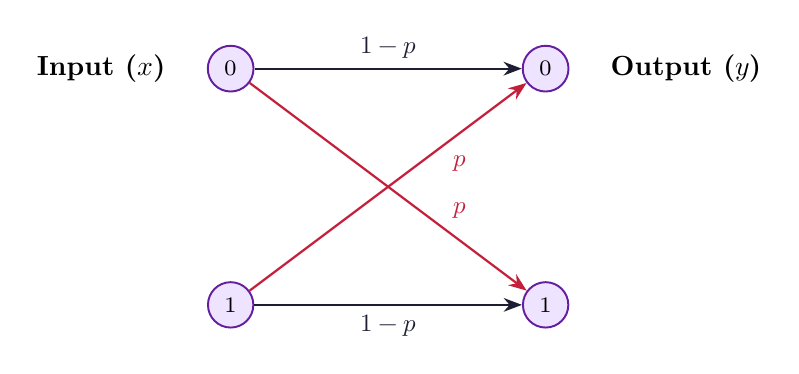
\begin{tikzpicture}[node distance=2.2cm and 3.2cm]
  \node[snode] (x0) at (0, 1.5) {$0$};
  \node[snode] (x1) at (0, -1.5) {$1$};
  \node[snode] (y0) at (4, 1.5) {$0$};
  \node[snode] (y1) at (4, -1.5) {$1$};

  \draw[arrow] (x0) -- node[above, pos=0.5]{\small $1-p$} (y0);
  \draw[arrow] (x1) -- node[below, pos=0.5]{\small $1-p$} (y1);
  \draw[redarrow] (x0) -- node[above right, pos=0.7]{\small $p$} (y1);
  \draw[redarrow] (x1) -- node[below right, pos=0.7]{\small $p$} (y0);
  
  \node[left=0.4cm of x0] {\textbf{Input ($x$)}};
  \node[right=0.4cm of y0] {\textbf{Output ($y$)}};
\end{tikzpicture}
\end{tcolorbox}

\subsection{Maximum Likelihood (ML) Decoding}
An optimum decoder minimizes the probability of decoding error. The maximum likelihood decoding rule selects the codeword $c^{(i)}$ that maximizes the conditional probability $P(r \mid c^{(i)})$:
\[ P(r \mid c^{(i)}) = p^{d(r, c^{(i)})} (1-p)^{n-d(r, c^{(i)})} \]
Since $p < 0.5 \implies 1-p > p$, we can rewrite this by taking the logarithm:
\[ \ln P(r \mid c^{(i)}) = d(r, c^{(i)}) \ln \left(\frac{p}{1-p}\right) + n \ln(1-p) \]
Since $\ln(p/(1-p)) < 0$ for $p < 0.5$, maximizing $P(r \mid c^{(i)})$ is mathematically equivalent to minimizing the Hamming distance:
\[ \text{ML Decoding Rule:} \quad \text{Choose } c \in C \text{ that minimizes } d(r, c) \]
Thus, over a BSC, Maximum Likelihood decoding simplifies to \textbf{minimum distance decoding}.

% ===============================================================================
\section{Syndrome Decoding on Symmetric Channels}
% ===============================================================================

Instead of calculating the distance from $r$ to all $2^k$ codewords, we can use the parity check matrix to compute a \textbf{Syndrome} vector $S$.

\begin{tcolorbox}[defbox, title={\textbf{The Syndrome}}]
The syndrome of a received vector $r$ is defined as:
\[ S = r \cdot H^T \]
\end{tcolorbox}

\subsection{Properties of the Syndrome}
\begin{enumerate}[label=\textbf{\arabic*.}, leftmargin=*, itemsep=3pt]
  \item $S = \mathbf{0}$ if and only if $r$ is a valid codeword.
  \item The syndrome depends \textbf{only on the error pattern} $e$, not on the transmitted codeword $c$:
    \[ S = r \cdot H^T = (c \oplus e) \cdot H^T = (c \cdot H^T) \oplus (e \cdot H^T) = \mathbf{0} \oplus (e \cdot H^T) = e \cdot H^T \]
  \item Two received vectors $r_1$ and $r_2$ have the same syndrome if and only if they differ by a valid codeword.
\end{enumerate}

\subsection{The Standard Array and Coset Leaders}
A standard array partitions the $2^n$ possible received vectors into a table of $2^{n-k}$ rows (called \textbf{cosets}) and $2^k$ columns.

\textbf{Standard Array Construction Algorithm:}\par\noindent
\begin{enumerate}[leftmargin=*, itemsep=3pt]
  \item Place all $2^k$ valid codewords in the first row, starting with the all-zero codeword $c_0 = \mathbf{0}$ on the far left.
  \item From the remaining unused vectors in $V_n$, choose a vector $e_1$ of minimum weight. Place it in the first column of the second row. This vector is the \textbf{coset leader}.
  \item Fill the second row by adding the coset leader $e_1$ to each codeword: $e_1 \oplus c_i$.
  \item Repeat this process: choose a minimum weight unused vector $e_j$ as the next coset leader, and fill the row with $e_j \oplus c_i$, until all $2^n$ vectors are placed.
\end{enumerate}

\begin{tcolorbox}[tikzbox, title={Standard Array Layout}]
{\renewcommand{\arraystretch}{1.5}%
\begin{tabularx}{\linewidth}{|>{\centering\arraybackslash}X|>{\centering\arraybackslash}X|>{\centering\arraybackslash}X|>{\centering\arraybackslash}X|>{\centering\arraybackslash}X|}
\hline
\textbf{Coset Leader ($e_j$)} & \textbf{Codeword $c_0=\mathbf{0}$} & \textbf{Codeword $c_1$} & \dots & \textbf{Codeword $c_{2^k-1}$} \\
\hline
$e_0 = \mathbf{0}$ & $\mathbf{0}$ & $c_1$ & \dots & $c_{2^k-1}$ \\
\hline
$e_1$ & $e_1$ & $e_1 \oplus c_1$ & \dots & $e_1 \oplus c_{2^k-1}$ \\
\hline
\vdots & \vdots & \vdots & \ddots & \vdots \\
\hline
$e_{2^{n-k}-1}$ & $e_{2^{n-k}-1}$ & $e_{2^{n-k}-1} \oplus c_1$ & \dots & $e_{2^{n-k}-1} \oplus c_{2^k-1}$ \\
\hline
\end{tabularx}}
\end{tcolorbox}

Each row (coset) corresponds to a unique syndrome. The coset leader is the \textbf{most likely error pattern} for that syndrome because it has the minimum weight in its coset.

\subsection{Syndrome Decoding Algorithm}
\begin{tcolorbox}[formulabox, title={\textbf{Syndrome Decoding Steps}}]
\begin{enumerate}[label=\textbf{Step \arabic*:}, leftmargin=2.0cm, itemsep=2pt]
  \item Compute the syndrome of the received vector: $S = r \cdot H^T$.
  \item Find the coset leader $e$ that matches this syndrome: $e \cdot H^T = S$.
  \item Correct the received vector to obtain the decoded codeword:
    \[ \hat{c} = r \oplus e \]
\end{enumerate}
\end{tcolorbox}

% ===============================================================================
\section{Hamming Codes}
% ===============================================================================

Hamming codes are a class of single-error-correcting linear block codes. For any integer $m \ge 2$, there exists a Hamming code with the following parameters:

\begin{tcolorbox}[defbox, title={\textbf{Hamming Code Parameters}}]
\begin{itemize}[leftmargin=*, itemsep=3pt, topsep=0pt]
  \item \textbf{Parity bits:} $n - k = m$
  \item \textbf{Code length:} $n = 2^m - 1$
  \item \textbf{Message length:} $k = 2^m - 1 - m$
  \item \textbf{Minimum distance:} $d_{min} = 3$
  \item \textbf{Error Correction:} Corrects all single errors ($t_c = 1$).
\end{itemize}
\end{tcolorbox}

\subsection{Structure of the Parity Check Matrix}
The parity check matrix $H$ of a Hamming code has $m$ rows and $2^m - 1$ columns. The columns of $H$ consist of all possible non-zero binary $m$-tuples, arranged in any order. In a systematic Hamming code:
\[ H = [P^T \mid I_m] \]
where the columns of $P^T$ consist of all non-zero binary $m$-tuples with weight $\ge 2$.

\subsection{Decoding of Hamming Codes}
When a single error occurs at position $i$, the received vector is $r = c \oplus e_i$, where $e_i$ has a $1$ at index $i$ and zeros elsewhere. The syndrome is:
\[ S = r \cdot H^T = (c \oplus e_i) \cdot H^T = e_i \cdot H^T = h_i^T \]
where $h_i^T$ is the transpose of the $i$-th column of $H$. Therefore, the syndrome $S$ is \textbf{identical to the column of $H$ corresponding to the error location}. If the columns of $H$ are arranged in order of their decimal equivalents, $S$ directly represents the index of the corrupted bit in binary.

% ===============================================================================
\section{Weight Enumerators and McWilliams Identities}
% ===============================================================================

The performance of a block code is determined by its \textbf{Weight Distribution}. Let $A_i$ be the number of codewords in $C$ with Hamming weight $i$. The set $\{A_0, A_1, \dots, A_n\}$ is the weight spectrum of the code.

\subsection{The Weight Enumerator Polynomial}
The weight distribution can be expressed as a polynomial:
\begin{tcolorbox}[defbox, title={\textbf{Weight Enumerator Polynomial}}]
\[ A(z) = \sum_{i=0}^n A_i z^i = A_0 + A_1 z + A_2 z^2 + \dots + A_n z^n \]
where $A_0 = 1$ (the all-zero codeword).
\end{tcolorbox}

\subsection{The McWilliams Identities}
The McWilliams identities relate the weight enumerator polynomial $A(z)$ of a linear block code $C$ of length $n$ to the weight enumerator polynomial $A^\perp(z)$ of its \textbf{dual code} $C^\perp$. The dual code $C^\perp$ is the set of all vectors orthogonal to every codeword in $C$, having dimension $n-k$ and generator matrix $H$.

\begin{tcolorbox}[formulabox, title={\textbf{McWilliams Identity Theorem}}]
For a binary $[n, k]$ linear code $C$ with weight enumerator $A(z)$ and dual code $C^\perp$ with weight enumerator $A^\perp(z)$:
\[ A^\perp(z) = \frac{1}{2^k} (1+z)^n A\left( \frac{1-z}{1+z} \right) \]
Alternatively, writing as a homogeneous polynomial in two variables $x$ and $y$:
\[ W_{C^\perp}(x, y) = \frac{1}{2^k} W_C(x+y, x-y) \]
\end{tcolorbox}
This identity is useful because it allows us to find the weight distribution of a code with large $k$ by analyzing its dual code which has a smaller dimension $n-k$ (e.g., finding the weight distribution of a $(127, 120)$ Hamming code by analyzing its $(127, 7)$ dual code).

% ===============================================================================
\section{Perfect Codes}
% ===============================================================================

For any block code correcting up to $t$ errors, the sphere of radius $t$ centered around each codeword must be disjoint. The total volume of these spheres cannot exceed the size of the vector space $2^n$.

\subsection{The Hamming Bound (Sphere-Packing Bound)}
The number of vectors in a sphere of radius $t$ in $V_n$ is:
\[ V(n, t) = \sum_{i=0}^t \binom{n}{i} \]
For $2^k$ codewords, we must have:
\[ 2^k \sum_{i=0}^t \binom{n}{i} \le 2^n \implies \sum_{i=0}^t \binom{n}{i} \le 2^{n-k} \]

\begin{tcolorbox}[defbox, title={\textbf{Perfect Code Definition}}]
A block code is a \textbf{Perfect Code} if it satisfies the Hamming bound with equality:
\[ 2^k \sum_{i=0}^t \binom{n}{i} = 2^n \]
In a perfect code, every vector in the space $V_n$ lies in exactly one sphere of radius $t$ around a codeword. There are no "wasted" vectors that cannot be corrected.
\end{tcolorbox}

\subsection{Examples of Perfect Codes}
Only a few families of perfect codes exist:
\begin{enumerate}[label=\textbf{\arabic*.}, leftmargin=*, itemsep=3pt]
  \item \textbf{Single-Error-Correcting Hamming Codes ($t=1$):}
    Satisfy: $1 + n = 2^{n-k} \implies 1 + (2^m - 1) = 2^m \quad \checkmark$
  \item \textbf{The Binary Golay Code ($[23, 12, 7]$):}
    Corrects $t=3$ errors.
    \[ \sum_{i=0}^3 \binom{23}{i} = 1 + 23 + 253 + 1771 = 2048 = 2^{11} = 2^{23-12} \quad \checkmark \]
  \item \textbf{The Ternary Golay Code ($[11, 6, 5]$):}
    Defined over GF(3), corrects $t=2$ errors.
    \[ \sum_{i=0}^2 \binom{11}{i} 2^i = 1 + 11(2) + 55(4) = 1 + 22 + 220 = 243 = 3^5 = 3^{11-6} \quad \checkmark \]
  \item \textbf{Trivial Perfect Codes:} The whole space ($d_{min}=1$), and binary repetition codes of odd length $n$ ($d_{min}=n, t = (n-1)/2$).
\end{enumerate}

% ═══════════════════════════════════════════════════════════════════════════════
% QUICK REVISION PAGE
% ═══════════════════════════════════════════════════════════════════════════════
\newpage
\begin{center}
  {\large\bfseries\color{myred} Quick Revision --- Module 1}\\[3pt]
  {\small\color{mydark} Linear Block Codes $|$ PE-EC801C}
\end{center}
\noindent{\color{myred}\rule{\linewidth}{1.2pt}}
\vspace{4pt}

\begin{tcolorbox}[formulabox, title={\textbf{Key Formulas and Metrics at a Glance}}]
\renewcommand{\arraystretch}{1.35}
\begin{tabularx}{\linewidth}{B{5.0cm} X}
Code Rate & $R = k/n$ \\[4pt]
Hamming Distance & $d(x, y) = w(x \oplus y)$ \\[4pt]
Error Correction Limit & $t_c = \lfloor (d_{min}-1)/2 \rfloor$ \\[4pt]
Systematic Generator Matrix & $G = [I_k \mid P]$ \\[4pt]
Parity Check Matrix & $H = [P^T \mid I_{n-k}]$ \\[4pt]
Orthogonality Condition & $G \cdot H^T = \mathbf{0} \pmod 2$ and $c \cdot H^T = \mathbf{0}$ \\[4pt]
Syndrome Vector & $S = r \cdot H^T = e \cdot H^T$ \\[4pt]
Hamming Bound (Sphere-Packing) & $2^k \sum_{i=0}^t \binom{n}{i} \le 2^n$ \\[4pt]
McWilliams Identity & $A^\perp(z) = \frac{1}{2^k} (1+z)^n A\left( \frac{1-z}{1+z} \right)$ \\[4pt]
Hamming Code Parameters & Length $n = 2^m-1$, Info bits $k = 2^m-1-m$, $d_{min}=3$
\end{tabularx}
\end{tcolorbox}

\vspace{6pt}

\begin{tcolorbox}[defbox, title={\textbf{One-Line Definitions}}]
\begin{itemize}[leftmargin=*, itemsep=3pt, topsep=0pt]
  \item \textbf{Linear Block Code:} A code where the modulo-2 sum of any two codewords is also a valid codeword.
  \item \textbf{Minimum Distance ($d_{min}$):} The smallest Hamming distance between any two distinct codewords in a code.
  \item \textbf{Syndrome:} A vector calculated as $r \cdot H^T$ that indicates if errors occurred and helps locate them.
  \item \textbf{Coset Leader:} The vector with the smallest Hamming weight in a coset, representing the most likely error.
  \item \textbf{Hamming Code:} A class of perfect single-error-correcting codes with minimum distance $d_{min} = 3$.
  \item \textbf{Perfect Code:} A code that satisfies the Hamming (sphere-packing) bound with strict equality.
  \item \textbf{Dual Code ($C^\perp$):} The set of all vectors orthogonal to every codeword in the original code $C$.
  \item \textbf{Binary Symmetric Channel:} A binary input/output channel where bit-flip probability is equal for $0$ and $1$.
\end{itemize}
\end{tcolorbox}

\newpage

\begin{tcolorbox}[exambox, title={\textbf{Frequently Asked / Viva Questions}}]
\begin{enumerate}[topsep=0pt, label=\textbf{Q\arabic*.}, itemsep=5pt]
  \item \Q{What is the difference between systematic and non-systematic codes?}
    In systematic codes, the message bits are placed directly at the beginning or end of the codeword, making extraction trivial. In non-systematic codes, message and parity bits are interleaved or mathematically combined throughout the codeword.
  \item \Q{Prove that $d_{min} = w_{min}$ for linear block codes.}
    For linear block codes, if $c_1, c_2 \in C$ are codewords, then $c_1 \oplus c_2 = c_3 \in C$ is also a codeword. The distance is $d(c_1, c_2) = w(c_1 \oplus c_2) = w(c_3)$. Thus, minimizing distance between distinct codewords is equivalent to finding the minimum weight of non-zero codewords.
  \item \Q{What is the physical significance of the syndrome vector?}
    The syndrome represents the parity-check violations of the received vector. Because $S = e \cdot H^T$, it depends strictly on the channel error pattern, not on the transmitted data, allowing isolated error isolation.
  \item \Q{Explain the ML decoding criteria over a Binary Symmetric Channel.}
    Maximum Likelihood decoding selects the codeword that maximizes $P(r \mid c)$. On a BSC with crossover probability $p < 0.5$, this probability increases as the distance $d(r, c)$ decreases. Thus, ML decoding reduces to minimum Hamming distance decoding.
  \item \Q{Why are Hamming codes considered perfect codes?}
    Hamming codes have $d_{min}=3$, meaning they correct $t=1$ error. They satisfy the sphere-packing bound with equality since $\sum_{i=0}^1 \binom{n}{i} = 1 + n = 1 + 2^m - 1 = 2^m = 2^{n-k}$, leaving no unused vectors.
  \item \Q{What is the role of a standard array in syndrome decoding?}
    A standard array groups all possible $2^n$ received vectors into $2^{n-k}$ cosets. Each coset shares the same syndrome, and the coset leader (first vector of the row) is chosen as the minimum-weight error pattern for correction.
  \item \Q{State the McWilliams identities and explain their utility.}
    The McWilliams identities relate the weight enumerator polynomial of a linear code to that of its dual code: $A^\perp(z) = 2^{-k}(1+z)^n A((1-z)/(1+z))$. This allows for the simplified calculation of the weight spectrum of high-rate codes (large $k$) by analyzing their lower-dimension dual codes.
  \item \Q{What is the Golay code, and why is it important?}
    The binary Golay code is a $[23, 12, 7]$ perfect code that corrects all patterns of up to $3$ random errors. It is the only known binary perfect code that corrects multiple errors ($t > 1$) besides repetition codes.
  \item \Q{Can a linear block code correct more errors than its minimum distance implies?}
    No. A code can guarantee the correction of all error patterns of weight up to $t = \lfloor(d_{min}-1)/2\rfloor$. While it may correct some specific patterns of weight $> t$, it cannot correct all of them.
  \item \Q{What happens if the syndrome matches no single column in a Hamming parity check matrix?}
    In a Hamming code, if the syndrome is non-zero but doesn't match a column representing a single-bit error (which is impossible since columns represent all non-zero $m$-tuples), it indicates that more than one error has occurred, leading to decoding failure.
\end{enumerate}
\tcbset{after={\color{black}}}
\end{tcolorbox}

\vspace{6pt}

\begin{tcolorbox}[tikzbox, title={\textbf{Comparison of Perfect and Near-Perfect Block Codes}}]
\renewcommand{\arraystretch}{1.45}
\begin{tabularx}{\linewidth}{|B{3.2cm}|Y|Y|Y|}
\hline
\textbf{Code Type} & \textbf{Parameters $[n, k, d_{min}]$} & \textbf{Error Correction ($t$)} & \textbf{Perfect Status} \\
\hline
Hamming Codes & $[2^m-1, 2^m-1-m, 3]$ & $t = 1$ & Perfect \\
\hline
Binary Golay Code & $[23, 12, 7]$ & $t = 3$ & Perfect \\
\hline
Ternary Golay Code & $[11, 6, 5]$ & $t = 2$ & Perfect \\
\hline
Repetition Codes & $[n, 1, n]$ ($n$ odd) & $t = (n-1)/2$ & Perfect (Trivial) \\
\hline
\end{tabularx}
\end{tcolorbox}

\end{document}
